Σε αυτή την ανάλυση συγκρίνεται η υπολογισμένη θερμοκρασία που παράγει το μοντέλο της εργασίας έναντι των μετρημένων χρονοσειρών της θερμοκρασίας των \textit{Tremblett \& Limebeer} \cite{Tremlett2016} κατά την εξέλιξη ενός γύρου. Έπειτα, εφαρμόζεται η ρουτίνα του κεφαλαίου \ref{sec:parameterFitting} με σκοπό τη βελτιστοποίηση των παραμέτρων του θερμοδυναμικού μοντέλου προς βαθμονόμηση με πειραματικά δεδομένα.

\begin{figure}[htbp!]
    \centering
    \begin{subfigure}[t]{0.48\textwidth}
        \centering
        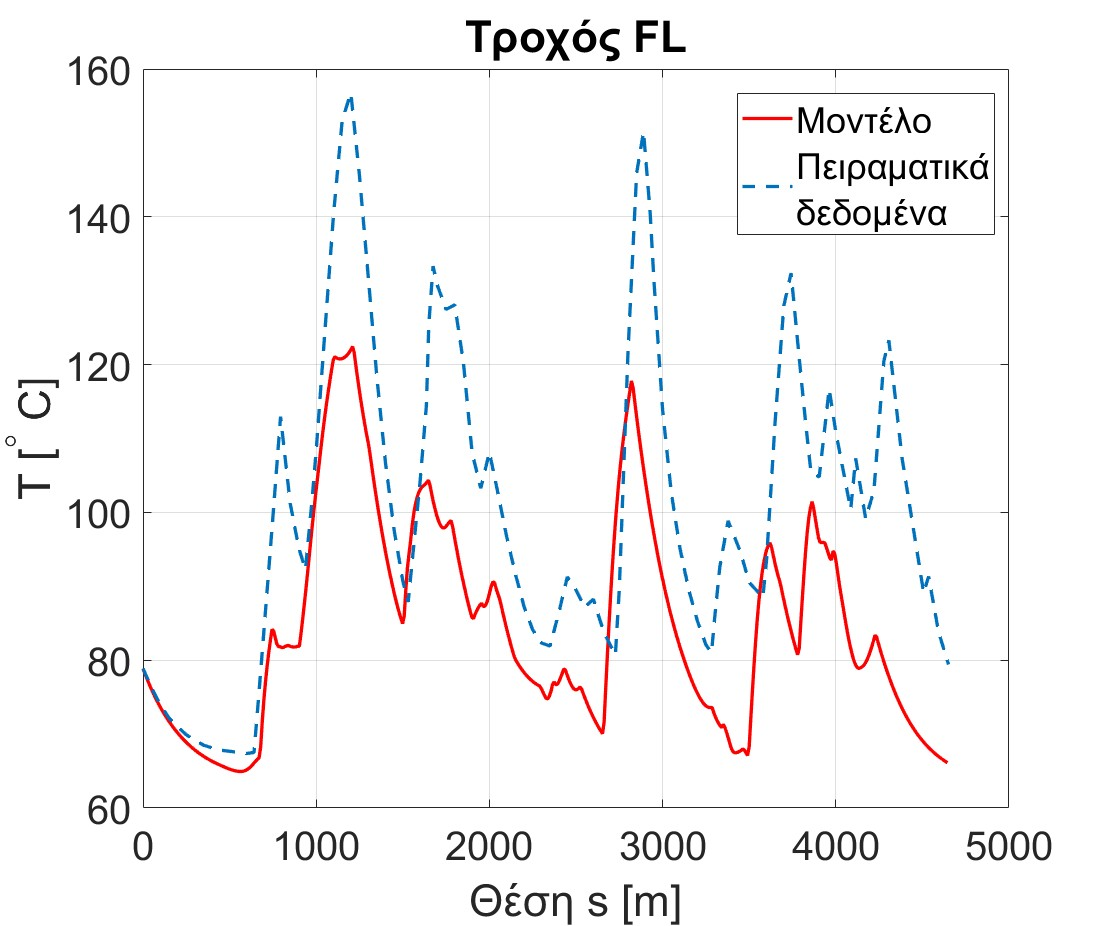
\includegraphics[width=\textwidth]{figures/FL_original_stateSolver_vs_Track.jpg}
    \end{subfigure}
    \hfill
    \begin{subfigure}[t]{0.48\textwidth}
        \centering
        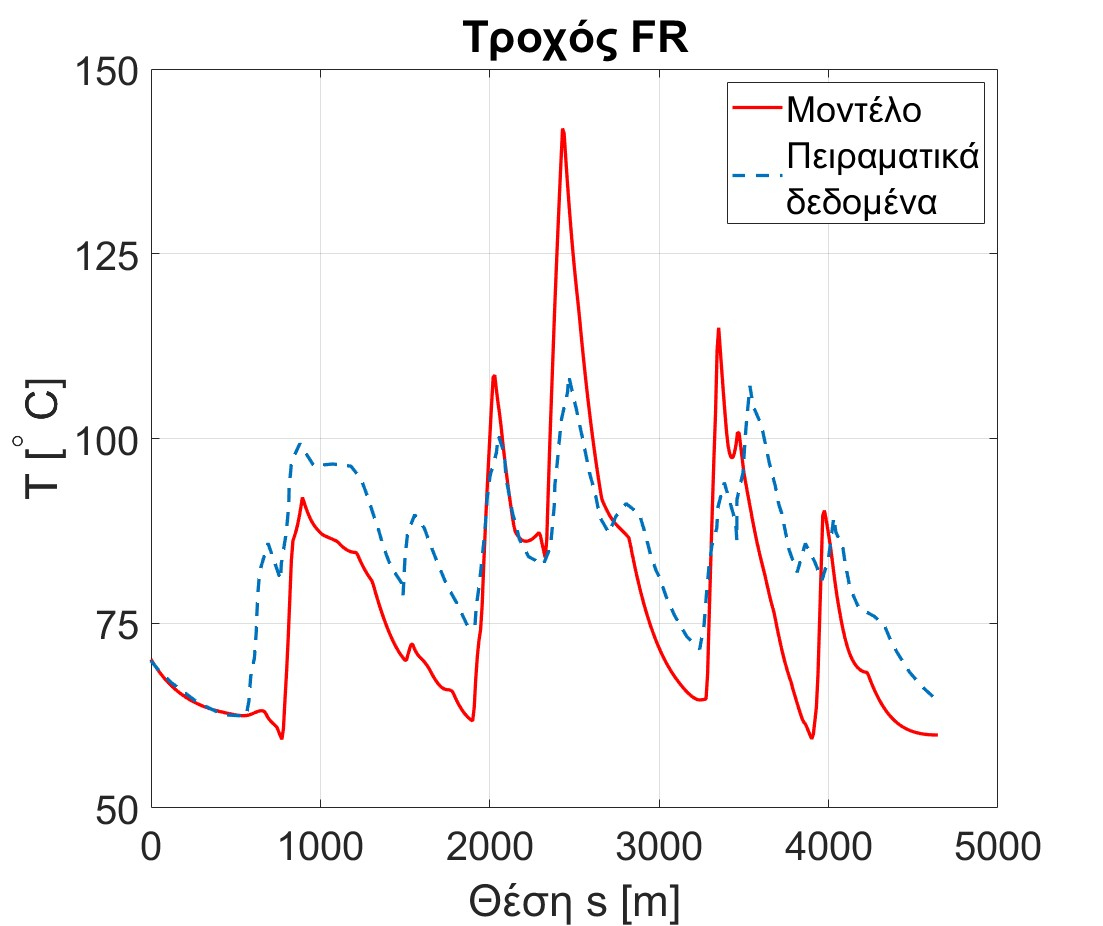
\includegraphics[width=\textwidth]{figures/FR_original_stateSolver_vs_Track.jpg}
    \end{subfigure}

    \vspace{0.5em}

    \begin{subfigure}[t]{0.48\textwidth}
        \centering
        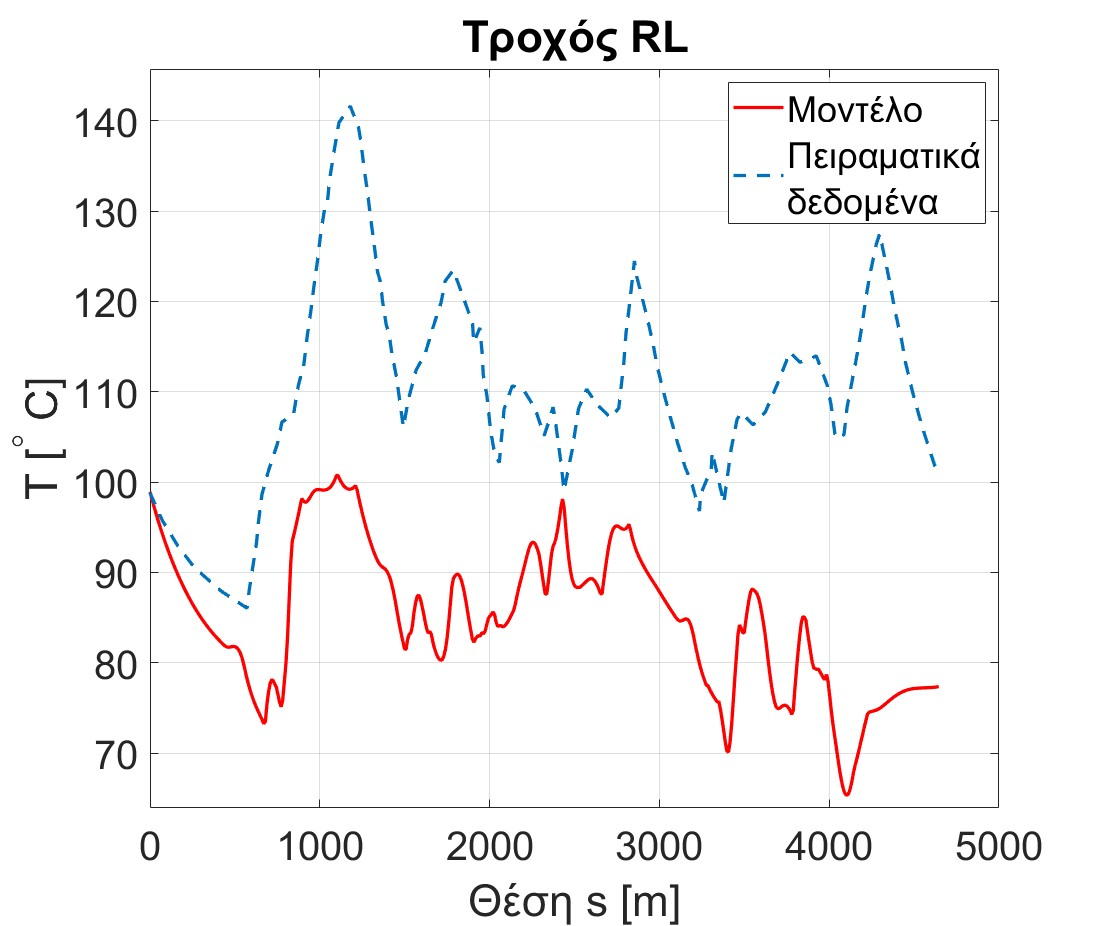
\includegraphics[width=\textwidth]{figures/RL_original_stateSolver_vs_Track.jpg}
    \end{subfigure}
    \hfill
    \begin{subfigure}[t]{0.48\textwidth}
        \centering
        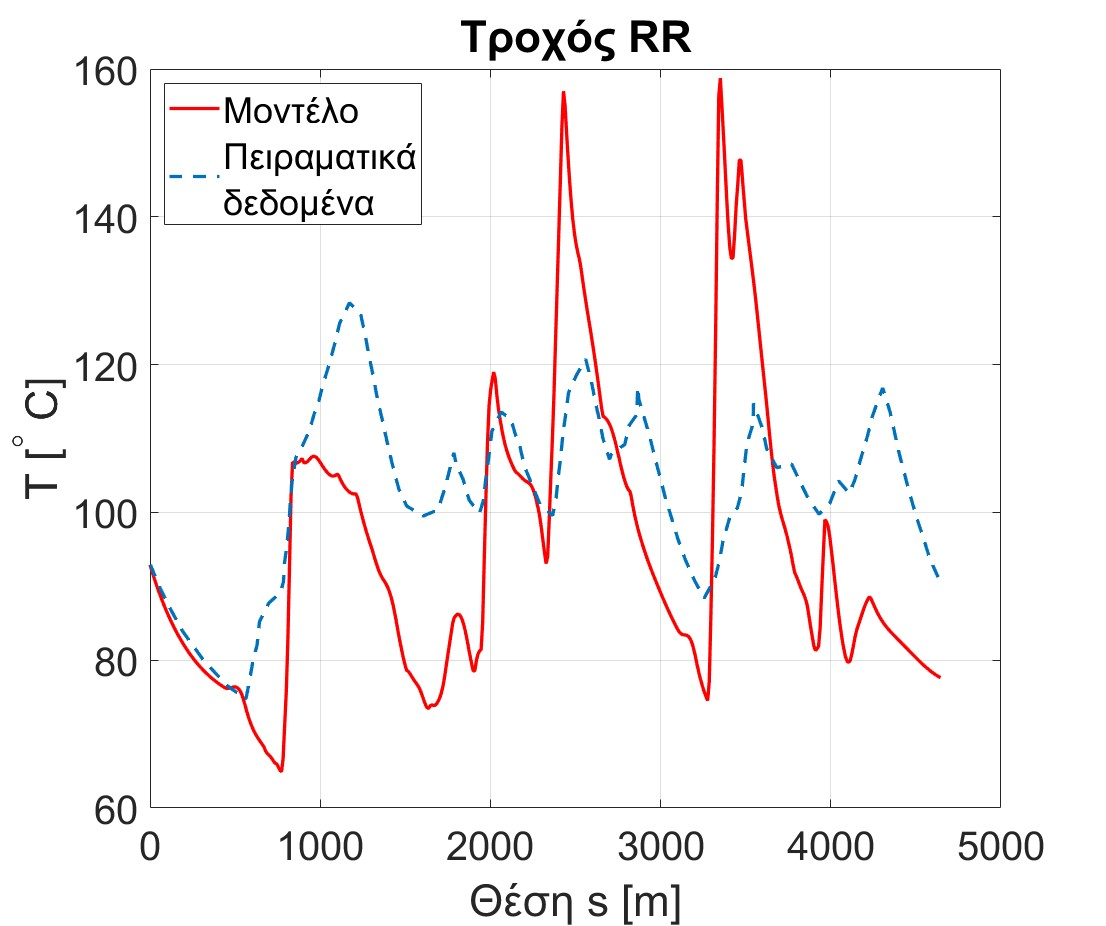
\includegraphics[width=\textwidth]{figures/RR_original_stateSolver_vs_Track.jpg}
    \end{subfigure}
    \caption{Σύγκριση θερμοκρασίας μοντέλου με πειραματική σε γύρο της πίστας \textit{Circuit de Barcelona - Catalunya}}
    \label{fig:defaultTemperaturesVsTests}
\end{figure}